\chapter{Vzorkování odraženého signálu}
Má-li být doržen Nyquistův vzorkovací teorém, je nezbytné vzorkovat budicí a odražený signál na nejméně dvakrát větší frekvenci, než se nachází nejvyšší frekvenční složka měřených signálů. Vybraný zdroj budicího signálu má šířku frekvenčního pásma až \SI{9}{\giga\hertz}, je tedy nezbytné, aby vzorkovač byl schopen vzorkovat alespoň na \SI{18}{\gigasample}. Tento vztah platí při zanedbání frekvenční charakteristiky vzorkovače, který se může chovat jako dolní propust, a tedy minimální vzorkovací frekvence může být nižší. Takovýmto vzorkovacím frekvencím se však blíží jen Flash \acrshort{ADC}, které však při takovýchto rychlostech jsou nanejvýš osmibitové, tedy nabízejí dynamický rozsah nanejvýš \SI{48}{\deci\bel}. Nejrychlejší převodníky zatím (v roce 2019) nedosahují vzorkovacích frekvencí \SI{10}{\giga\hertz}. Pro rychlejší vzorkování se používá tzv. \gls{ADCinterleave}, tedy prokládání většího počtu převodníků. Pro přenos a zpracování dat z takto rychlých převodníků jsou potřeba i velmi rychlá FPGA, případně ještě signálové procesory. Tato metoda je ve výsledku v současné době velmi nákladná, navíc má malý dynamický rozsah.

Od doby prvních digitálních osciloskopů se používá technika známá jako vzorkování v \quotedblbase ekvivalentním čase\textquotedblleft\. Tato metoda spočívá ve vzorkování periodického signálu přes větší množství jeho period, přičemž postupně se doplňují změřené body, dokud nejsou nalezeny všechny body měřeného průběhu. Hlavní nevýhoda tohoto postupu je nemožnost vzorkování jednorázových signálů (např. šum). Zásadní výhoda tohoto postupu je ovšem možnost částečně potlačit rušení z okolí, jsou-li asynchronní vůči vzorkování. Případně je možné i zvětšit dynamický rozsah, je-li použit rychlý vzorkovač pro navzorkování signálu pro pomalejší vícebitový \acrshort{ADC}. Existují dva základní přístupy, jak provádět toto vzorkování:
\begin{itemize}
	\item
		\textbf{Náhodné vzorkování}\\*		
		Vzorky jsou odebírány neustále, je zaznamenáván časový rozdíl mezi spouštěcí událostí (zde začátek budicího signálu) a nejbližší následující periodou vzorkovacího hodinového signálu. Postupně se tak náhodně doplňují naměřené body, až vznikne dostatečně přesný obraz měřeného signálu. Tato metoda je vhodná například pro osciloskopy, protože zpravidla není možné synchronizovat přesně vzorkovací hodinový signál se spouštěcí událostí.
		
	\item
		\textbf{Postupné vzorkování}\\*
		Vzorky jsou odebírány při každé periodě měřeného průběhu tak, že jednotlivé odebrané vzorky jsou časově seřazeny. Toho se dá dosáhnout fázovým posouváním vzorkovacího hodinového signálu oproti spouštěcí události, což je možné udělat pomocí digitálních zpožďovacích linek nebo tak, že vzorkovací hodinový signál a budicí signál budou mít nepatrně jinou frekvenci \cite{vernierreflectometer}. První řešení může být jednodušší na implementaci, ale zpožďovací linka omezuje krok měření a maximální počet odebraných vzorků \cite{fpgadelaylinereflectometer}, \cite{simpledelaylinereflectometer}. Druhé řešení se dá vytvořit pomocí \acrshort{DDS} \cite{ddsfpgareflectometer} nebo fázového závěsu, který podporuje násobení nebo dělení frekvencí neceločíselným násobkem. Do nedávné doby nebylo řešení pomocí fázových závěsů praktické, protože vyžadovalo fázový závěs pro vytvoření vysokofrekvenční reference a další dva fázové závěsy pro vytvoření dvou rozdílných frekvencí. V posledních letech se však objevily fázové závěsy, které všechny tyto funkce (včetně \acrshort{VCO}) integrují do jediného integrovaného obvodu a prakticky vyžadují pouze kmitočtovou referenci v podobě krystalu nebo krystalového oscilátoru \cite{ADF4350datasheet} \cite{Si5351datasheet}.
\end{itemize}

\begin{figure}[htbp]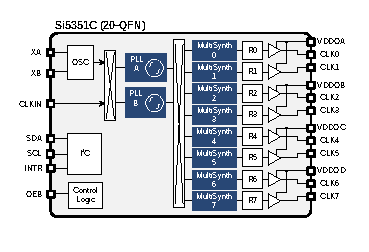
\includegraphics[width=\textwidth,keepaspectratio]{images/si5351_internal_architecture_overview.eps}\caption{Blokové zapojení \acrshort{PLL} Si5351 \cite{Si5351datasheet}.}\label{5351blockdiagram}\end{figure}

Vzhledem k existenci dostupných fázových závěsů umožňujících velkou integraci a miniaturizaci zapojení bylo zvoleno postupné vzorkování pomocí fázového závěsu. Vybraný fázový závěs Si5351 obsahuje v jednom pouzdře dva neceločíselné fázové závěsy \cite{Si5351datasheet}, dva vysokofrekvenční \acrshort{VCO} a osm výstupních neceločíselných děliček. Díky tomuto vývoji v integraci je možné celý hodinový generátor zmenšit do podoby jednoho integrovaného obvodu, jedinou potřebnou externí součástkou je krystal nebo krystalový oscilátor. Neceločíselná část násobiče frekvence umožňuje krok po $2^{{-20}}$ referenční frekvence, je tedy možné měnit podíl frekvencí hodinových signálů s krokem menším než \SI{1}{\ppm}. Při rozdílu frekvencí \SI{1}{\ppm} je počet vzorkovaných bodů celkem 1\,000\,000, což je počet bodů, který je prakticky nedosažitelný se zpožďovacími linkami.

\section{Obvodové řešení vzorkovače}
Pro měření je potřeba vzorkovač s velkou šířkou pásma, nezbytný je i malý \gls{aperturetime}. Historicky se pro tyto účely používaly diodové vzorkovače \cite{S-1manual} \cite{S-4manual}, příklad takového zapojení na obr. \ref{oscilloscopefrontend}. V dnešní době existují již dostatečně rychlé track-and-hold zesilovače, tedy zesilovače, které je možné řízeně zastavit, přičemž na jejich výstupu zůstane napětí, které se tam nacházelo v okamžiku vypnutí zesilovače. Jejich mezní kmitočet se pohybuje v současné době okolo \SI{8}{\giga\hertz}. Bohužel jsou oproti diodovým vzorkovačům velice nákladné.

\begin{figure}[htbp]\includegraphics[width=\textwidth,keepaspectratio]{images/oscilloscopefrontend.png}\caption{Praktické zapojení vzorkovacího můstku do \SI{1}{\giga\hertz}, převzato z \cite{oscilloscopefrontend}.}\label{oscilloscopefrontend}\end{figure}		

Diodové vzorkovače se používaly již v prvních digitálních osciloskopech a reflektometrech, protože jejich šířka použitelného frekvenčního pásma je omezena téměř výhradně sériovým dynamickým odporem diodového vzorkovače, velikostí vzorkovacího kondenzátoru a aperturovým časem. Aperturový čas je doba, po kterou trvá rozepnout vzorkovač, závisí zejména na kapacitě diody (bariérové i difuzní) a zapojení budiče, který diody rozepíná. Pro toto použití jsou zejména vhodné Schottkyho diody kvůli malé paralelní kapacitě a možnosti velice rychle diody rozepnout. Speciálně pro použití ve vzorkovačích se vyrábí přesné vyvážené diodové čtveřice \cite{HSMS282xdatasheet}, které umožňují silně potlačit průnik vzorkovacího buzení do vzorkovaného signálu, což umožňuje použití velmi malých vzorkovacích kondenzátorů, a tedy velkou šířku užitečného frekvenčního pásma takového vzorkovače.
	